\documentclass[12pt,accentcolor=tud2c, longdoc, colorback, bigchapter]{tudreport}
\usepackage[utf8]{inputenc}
\usepackage[ngerman]{babel}
\usepackage{amsmath}
\usepackage{amsfonts}
\usepackage{amssymb}
\usepackage{graphicx}
\usepackage{listings}
\usepackage{color}
\usepackage{numprint}
\usepackage[ngerman]{cleveref}
\usepackage{csquotes}
\usepackage{apacite}
\usepackage{svg}
\usepackage{pstricks}
\usepackage{float}
\usepackage{geometry}
\usepackage{microtype}

\selectlanguage{ngerman}
\graphicspath{{img/}}
\author{}
\title{Ein neues Reißverschlußsystem}
\subtitle{Projektkurs CE – SS 2017}
\subsubtitle{}

\begin{document}
\maketitle
\cleardoublepage
\pagenumbering{Roman}
\setcounter{page}{3}
\tableofcontents
\listoffigures
%\listoftables
% Eigentlicher Text mit arabischen Seitenzahlen
\cleardoublepage
\pagenumbering{arabic}
\setcounter{page}{1}
\chapter{Slick}
%Literaturverzeichnis
%\bibliographystyle{plaindin}
\bibliographystyle{apacite}
\bibliography{literatur}
%Appendix
\appendix
%\chapter{Anhang}
\section{UML Diagramme}
\subsection{Klassendiagramm}
\begin{figure}
	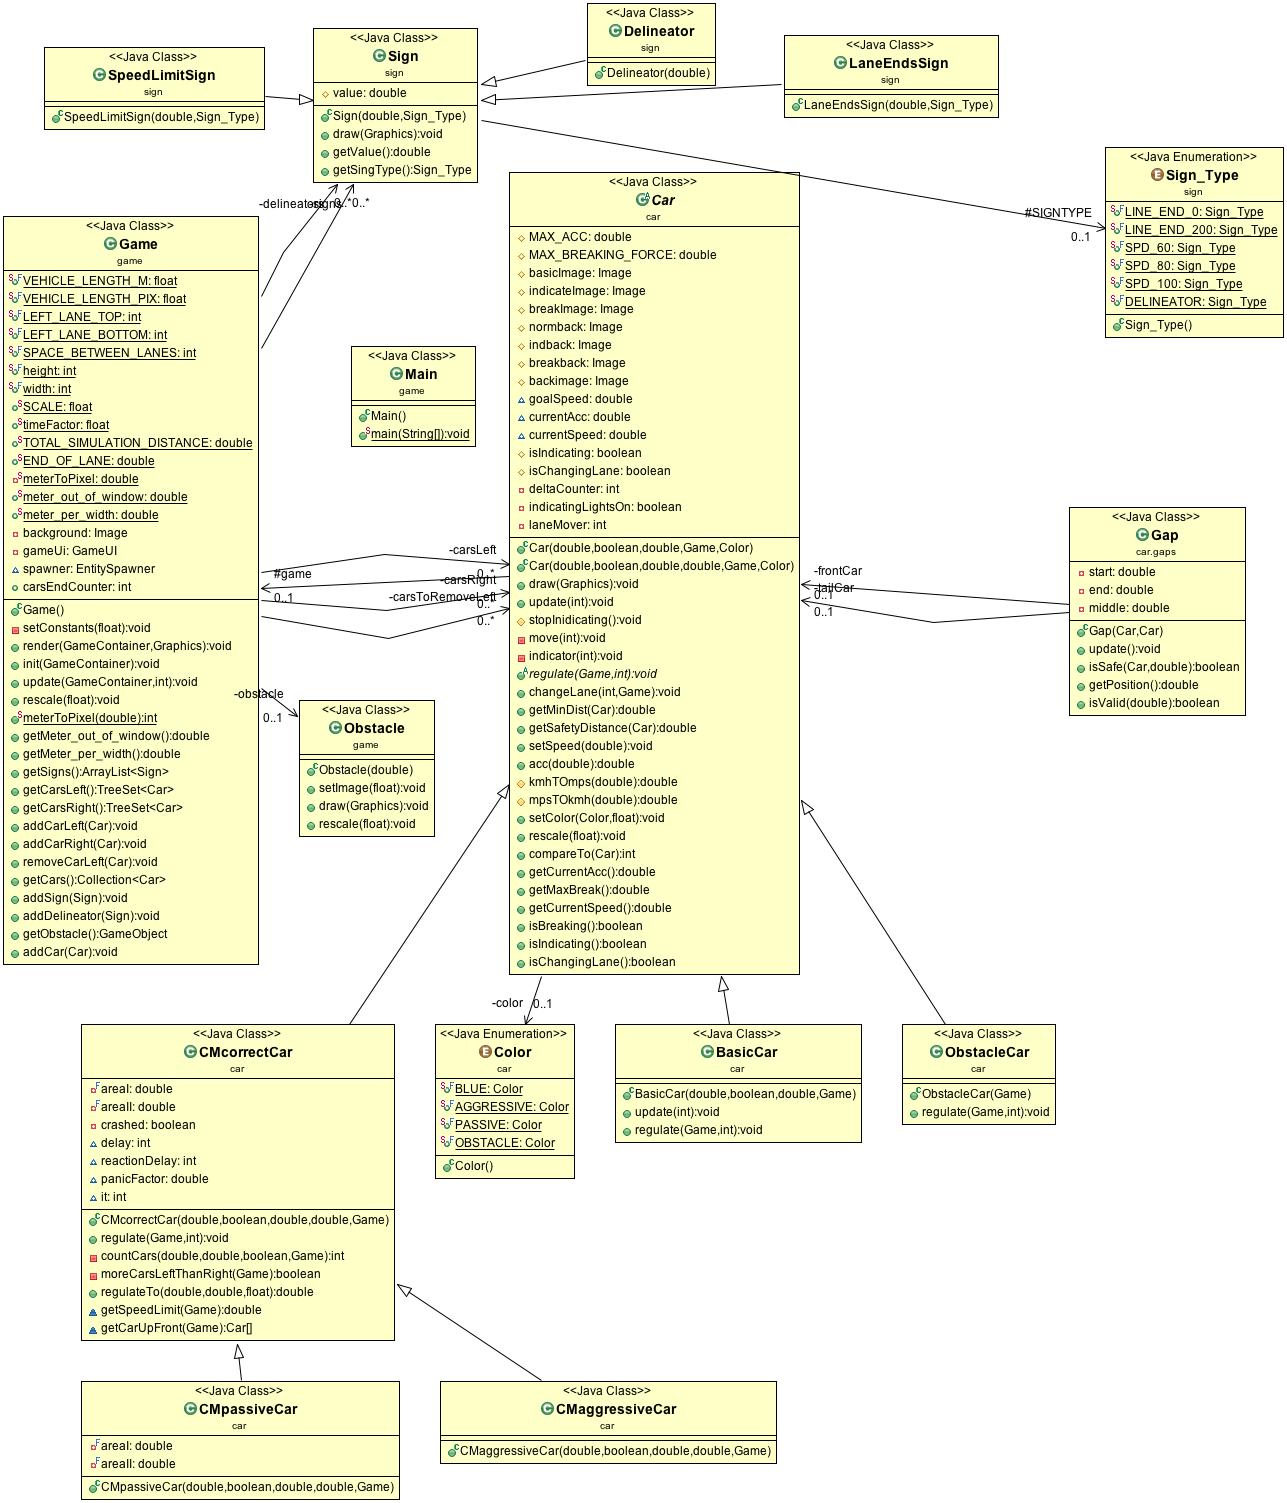
\includegraphics[width=\linewidth]{images/classuml.png}
	\caption{UML Klassendiagramm}
	\label{fig:umlclass}
	\end{figure}

\end{document}